%%%%%%%%%%%%%%%%%%%%%%%%%%%%%%%%%%%%%%%%%
% Academic Title Page
% LaTeX Template
% Version 2.0 (17/7/17)
%
% This template was downloaded from:
% http://www.LaTeXTemplates.com
%
% Original author:
% WikiBooks (LaTeX - Title Creation) with modifications by:
% Vel (vel@latextemplates.com)
%
% License:
% CC BY-NC-SA 3.0 (http://creativecommons.org/licenses/by-nc-sa/3.0/)
%
% Instructions for using this template:
% This title page is capable of being compiled as is. This is not useful for
% including it in another document. To do this, you have two options:
%
% 1) Copy/paste everything between \begin{document} and \end{document}
% starting at \begin{titlepage} and paste this into another LaTeX file where you
% want your title page.
% OR
% 2) Remove everything outside the \begin{titlepage} and \end{titlepage}, rename
% this file and move it to the same directory as the LaTeX file you wish to add it to.
% Then add \input{./<new filename>.tex} to your LaTeX file where you want your
% title page.
%
%%%%%%%%%%%%%%%%%%%%%%%%%%%%%%%%%%%%%%%%%

%----------------------------------------------------------------------------------------
%	PACKAGES AND OTHER DOCUMENT CONFIGURATIONS
%----------------------------------------------------------------------------------------

\documentclass[11pt]{article}

\usepackage[a4paper, total={6in, 8in}]{geometry}

\usepackage{multicol}

\usepackage[utf8]{inputenc} % Required for inputting international characters
\usepackage[T1]{fontenc} % Output font encoding for international characters

\usepackage{mathpazo} % Palatino font

\usepackage{graphicx}

\usepackage{minted}
\usemintedstyle{manni}

\usepackage{hyperref}
\hypersetup{
    colorlinks=true,
    linkcolor=blue,
    filecolor=magenta,
    urlcolor=cyan,
}

\begin{document}

%----------------------------------------------------------------------------------------
%	TITLE PAGE
%----------------------------------------------------------------------------------------

\begin{titlepage} % Suppresses displaying the page number on the title page and the subsequent page counts as page 1
  \newcommand{\HRule}{\rule{\linewidth}{0.5mm}} % Defines a new command for horizontal lines, change thickness here

  \center{} % Centre everything on the page

  %------------------------------------------------
  %	Headings
  %------------------------------------------------

  % Main heading such as the name of your university/college
  \textsc{\LARGE Swinburne University of Technology}\\[1.5cm]

  % Major heading such as course name
  \textsc{
    \Large
    Bachelor of Engineering\\
    (Software Engineering)\\
    (Honours)
  }\\[0.5cm]

  % Minor heading such as course title
  \textsc{\large ICT40010 Research Report A}\\[0.5cm]

  %------------------------------------------------
  %	Title
  %------------------------------------------------

  \HRule{}\\[0.4cm]

  % Title of your document
  {\huge\bfseries Technical Report}\\[0.2cm]

  \HRule{}\\[1.5cm]

  %------------------------------------------------
  %	Author(s)
  %------------------------------------------------

  \begin{minipage}{0.4\textwidth}
    \begin{flushleft}
      \large
      \textit{Author}\\
      D.J. \textsc{Holland}
    \end{flushleft}
  \end{minipage}
  {~}
  \begin{minipage}{0.4\textwidth}
    \begin{flushright}
      \large
      \textit{Supervisors}\\
      Dr.\ Clinton \textsc{Woodward}\\
      Dr.\ Charlotte \textsc{Pierce}
    \end{flushright}
  \end{minipage}

  % If you don't want a supervisor, uncomment the two lines below and comment the code above
  %{\large\textit{Author}}\\
  %John \textsc{Smith} % Your name

  %------------------------------------------------
  %	Date
  %------------------------------------------------

  \vfill\vfill\vfill % Position the date 3/4 down the remaining page

  {\large\today} % Date, change the \today to a set date if you want to be precise

  %------------------------------------------------
  %	Logo
  %------------------------------------------------

  %\vfill\vfill
  %\includegraphics[width=0.2\textwidth]{placeholder.jpg}\\[1cm] % Include a department/university logo - this will require the graphicx package

  %----------------------------------------------------------------------------------------

  \vfill % Push the date up 1/4 of the remaining page

\end{titlepage}

%----------------------------------------------------------------------------------------

\tableofcontents
\pagenumbering{gobble}
\newpage
\pagenumbering{arabic}

\newcommand{\boxy}[1]{\colorbox{gray!10}{\mintinline{text}{#1}}}

\setlength{\columnsep}{0.5cm}
\begin{multicols}{2}
  [
    \section{Introduction}
    TODO:\ introduction
  ]

  \section{Technology}

  \subsection{Rust}
  Rust is a systems prorgramming language that guarantees memeroy safety at compile time.
  Rust doesn't need a garbage collector so the performance is excellent with little to no overhead.
  There is zero-cost bidirectional interopability with C via the FFI\@;
  a basic requirement for communicating with OpenGL on the system.

  The modern Rust toolchain makes it trivial to have a fast and friendly developer experience.

  \subsection{OpenGL}
  OpenGL is the go-to cross-platform graphics API with a wealth of learning resources available.
  Using OpenGL and Rust enables the application to run on Windows, Mac OS, and Linux without much platform specific thought. OpenGL \boxy{4.1} is minumum target version as that is the latest version supported on Mac OS\@.

  Vulkan was considered, but due the increased complexity of properly implementing a Vulkan based application, OpenGL was the simpler choice.

  \subsection{VS Code}
  Continuing with cross-platform tools, VS Code is the text-editor/IDE of choice.
  Using the excellent rust-analyzer extension, it's a decent Rust IDE\@.
  With various other extensions, writing shader code and documentation is also pleasant.

  \subsection{GitHub}
  Several services on GitHub are used:
  \begin{itemize}
    \item It's the main git remote repository for the code
    \item Issues are tracked on there
    \item Projects, labels, and milestones help triage those issues
    \item Actions are used to build and test the code (CI)
    \item Pages is used to host this website which is deployed from Actions (CD).
  \end{itemize}

  \subsection{Vuepress}
  Vuepress is a static site generator particularly designed for writing technical documentation. It is what powers this website.

  \section{Foundation}

  \subsection{Crates}
  Rust's package manager, \textbf{Cargo}, allows code dependencies to be easily required by specifying them in a \boxy{Cargo.toml} file.
  In Rust-land, packages are known as \textbf{Crates}.

  Many crates are used in the application, with the most fundamental ones being outlined below.

  \subsection{gl}
  Unsafe bindings to raw OpenGL calls.
  This is what allows the application to interop with OpenGL on the system.
  If this crate didn't exist, then this application would have been written with C++ because generating function pointers for system APIs is not within the scope this project.

  \subsection{glutin}
  Manages windowing, events, and the OpenGL context.
  Another excellent create for cross-platform windowing and IO\@.
  The functions from the \textbf{gl} crate get loaded by the OpenGL context that \textbf{glutin} creates.

  \subsection{imgui}
  Immediate Mode Graphical User Interface.
  Creating UI is out of the scope of this project, IMGUI is an incredibly popular rendering-API-agnostic library for creating development tooling.
  This crate provides some safe abstraction as well as bindings to every IMGUI function.

  \subsection{nalgebra-glm}
  This crate is a subset of linear algebra tools from the \textbf{nalgebra} crate specifically for math used in graphics programming.

  \section{Architecture}

  \subsection{Modules}

  \subsubsection{Overview}
  Rust's module system provides an easy way to group code for readability, reuse, and privacy.
  The boxes in \textbf{Figure 1} are derivitive of the directory structure of the source code, with important modules having further explanation following.

  The application is split into two main projects:
  \begin{itemize}
    \item \textbf{Sandbox}: a binary application to run and demonstrate the Glamour library.
    \item \textbf{Glamour}: a library project containing all the rendering functionality.
  \end{itemize}

  \begin{figure}[H]
    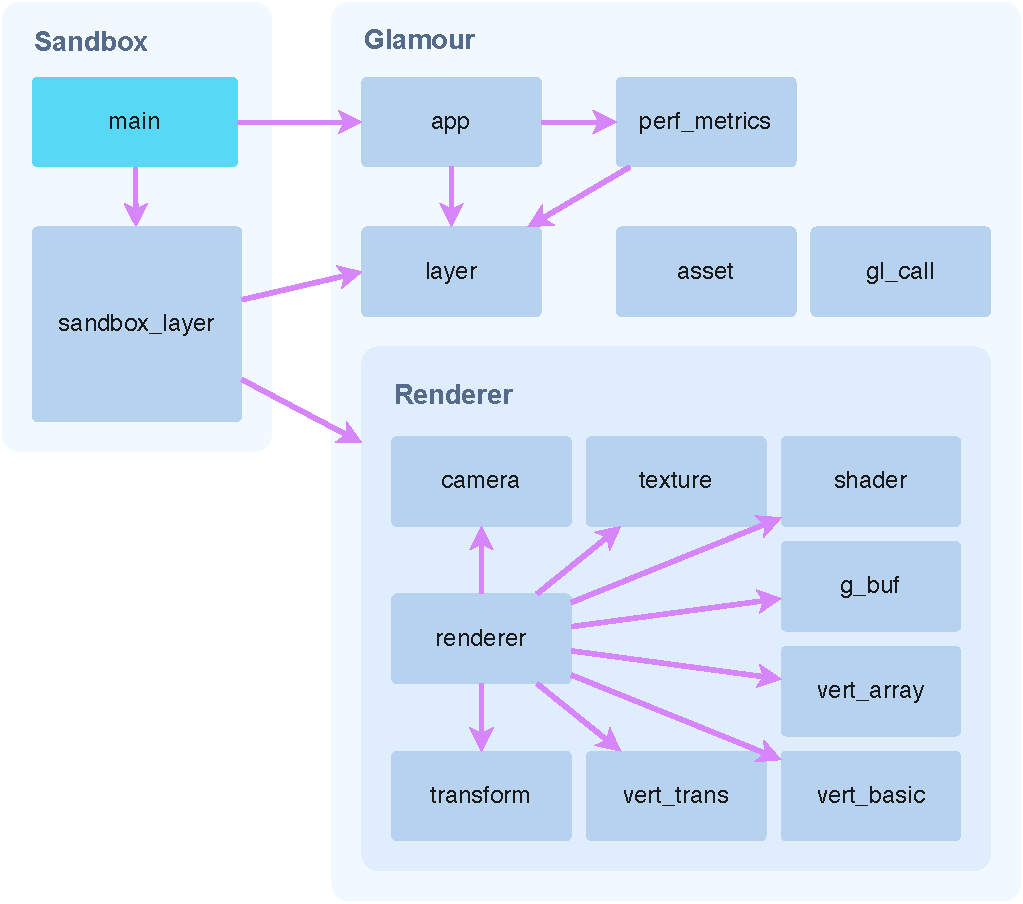
\includegraphics[width=1\columnwidth]{../module-graph.pdf}
    \caption[Module graph]{\emph{A simplified module and dependency graph for the application.}}\label{fig:module-graph}
  \end{figure}

  \subsubsection{app}
  The app module is responsible for managing the window, event loop, and OpenGL context.
  This is where layers are stored and processed.

  \subsubsection{layer}
  A layer is a trait (like an interface) that can handle events and do things on update loops.

  \subsubsection{asset}
  This module provides a way to load files from the `assets` folder, which is copied relative to the executable on build.

  \subsubsection{gl\_call}
  Since all the OpenGL functions are inherently \emph{unsafe}, the \boxy{gl_call!} macro will wrap a function and \emph{panic} if it errors, making OpenGL much easier to use.

  \subsubsection{renderer}
  This is what actually makes the draw calls.
  The renderer also manages the shaders, vertex arrays, and G-buffer, amongst other things.

  \subsection{Sandbox}
  The Sandbox project initialises an \textbf{app} instance and attaches a \textbf{sandbox\_layer} to it.
  The \textbf{sandbox\_layer} is responsible for instructing the \textbf{renderer} what to render, e.g., \emph{render 10,000 cubes at these randomly seeded positions from this camera angle}.

\end{multicols}

\section{Main Loop}

\subsection{Initialising}
The \boxy{main} function in Sandbox only contains 4 lines:
\begin{minted}{rust}
fn main() {
    let mut app = glamour::App::new("Glamour Sandbox", 1920, 1080);
    let sandbox_layer = SandboxLayer::new("SandboxLayer");
    app.push_layer(Box::new(sandbox_layer));
    app.run();
}
\end{minted}
Calling \boxy{glamour::App::new(title: &str, width: u32, height: u32)} will do the following:
\begin{itemize}
  \item Create a new event loop from the \boxy{glutin} crate to handle OS I/O
  \item Build a window with the supplied \boxy{title}, \boxy{width}, and \boxy{height}
  \item Load OpenGL within that window's context
  \item Load imgui
  \item Initialise the Layer stack.
\end{itemize}
After this point, layers can be pushed to the app, and then run.

\begin{multicols}{2}

  \subsection{Layer}
  A \boxy{Layer} is a basic trait to handle events of distinct parts of the application.
  Layers don't communicate with each other through the app, they're meant to be separate.
  There are only two layers used in the app:
  \begin{itemize}
    \item \boxy{PerfMetricsLayer} for reporting performance metrics
    \item \boxy{SandboxLayer} is a place to store all Sandbox related things.
  \end{itemize}
  \boxy{Layer} provides a few funtions that an implementation can use:
  \begin{itemize}
    \item \boxy{init()}
    \item \boxy{on_event()}
    \item \boxy{on_fixed_update()}
    \item \boxy{on_frame_update()}
    \item \boxy{on_imgui_update()}
  \end{itemize}

  Hopfully, those should be fairly self documentating.

  \subsection{Event Loop}
  Calling \boxy{app.run()} kickstarts the main event loop, which is responsible for
  \begin{itemize}
    \item Polling for events
    \item Managing fixed and frame updates
    \item Updating and rendering imgui
    \item Calling the each layer's \boxy{Layer} trait functions at the appropriate point
    \item Swapping the frame buffer to actually show the rendered image on the screen.
  \end{itemize}

  \subsection{AppContext}
  \boxy{App} also maintains a struct that holds the context of the application.
  This is \boxy{AppContext}, it provides some convenience to access things such as the window context and frame timings.
  This is passed to each \boxy{Layer} function.

  \section{Renderer}

  TODO: Details on the rendering pipeline, how OpenGL is used, and performance metrics.
  use lots of pictures here, it's the main visual element.

  \subsection{Pipeline}

  \subsubsection{Overview}

  \begin{figure}[H]
    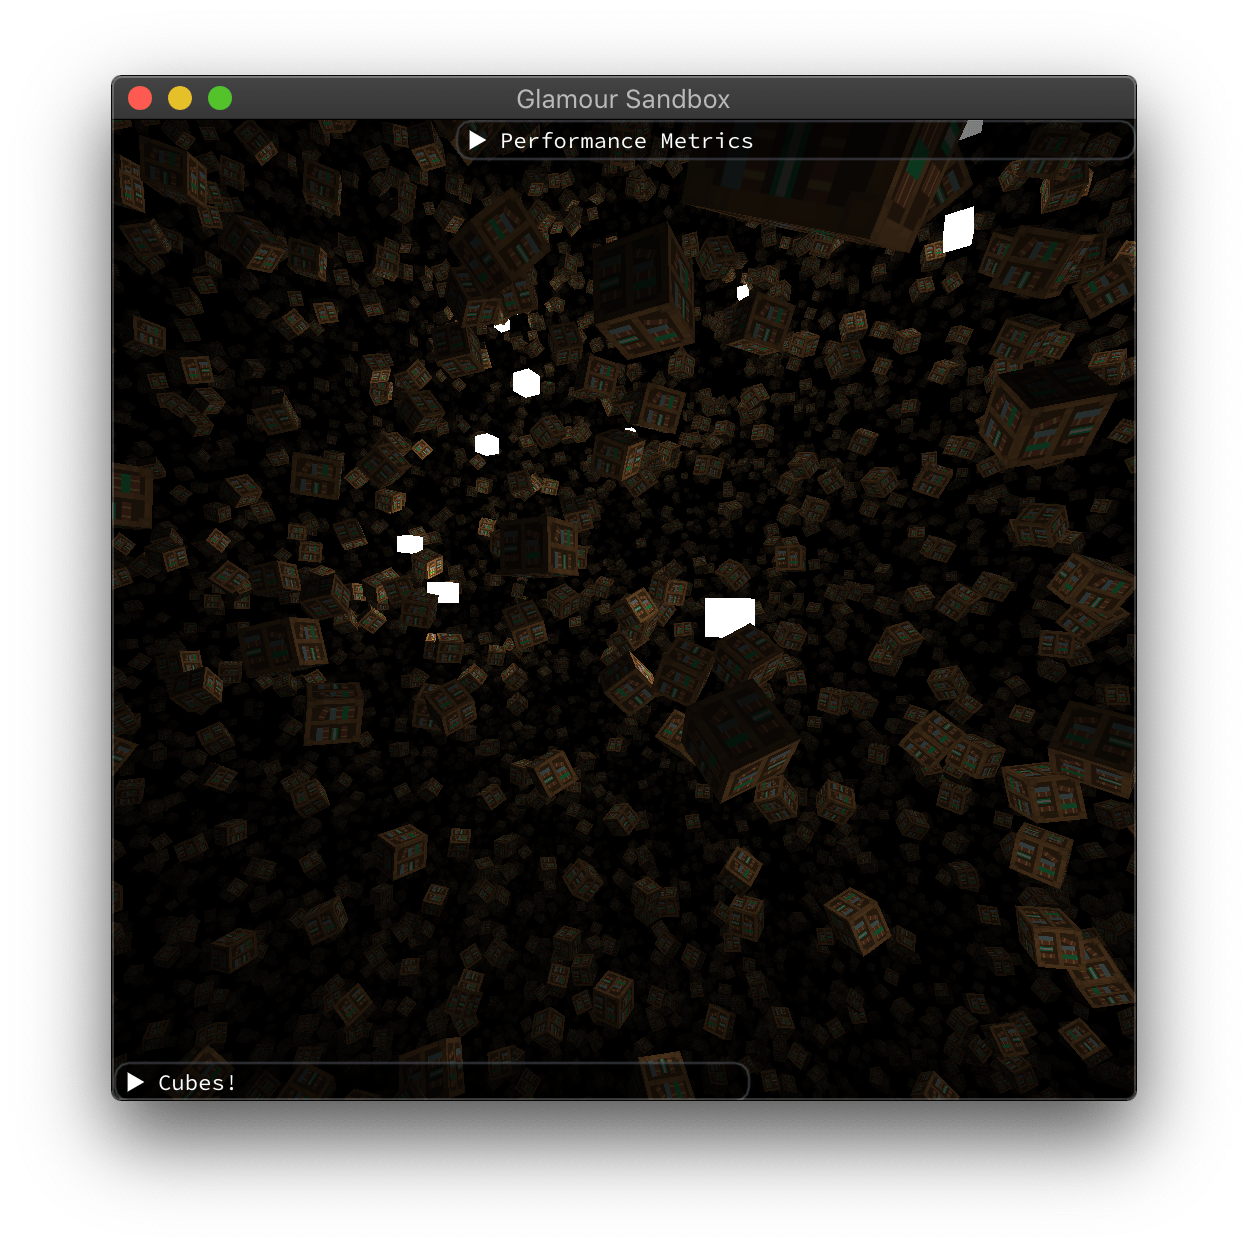
\includegraphics[width=1\columnwidth]{../sandbox.png}
    \caption[Sandbox screenshot]{
      \emph{
        Running the application results in the scene above.
        A bunch of rotating cubes, with lights travelling around the world.
      }
    }\label{fig:sandbox-screenshot}
  \end{figure}

  \begin{figure}[H]
    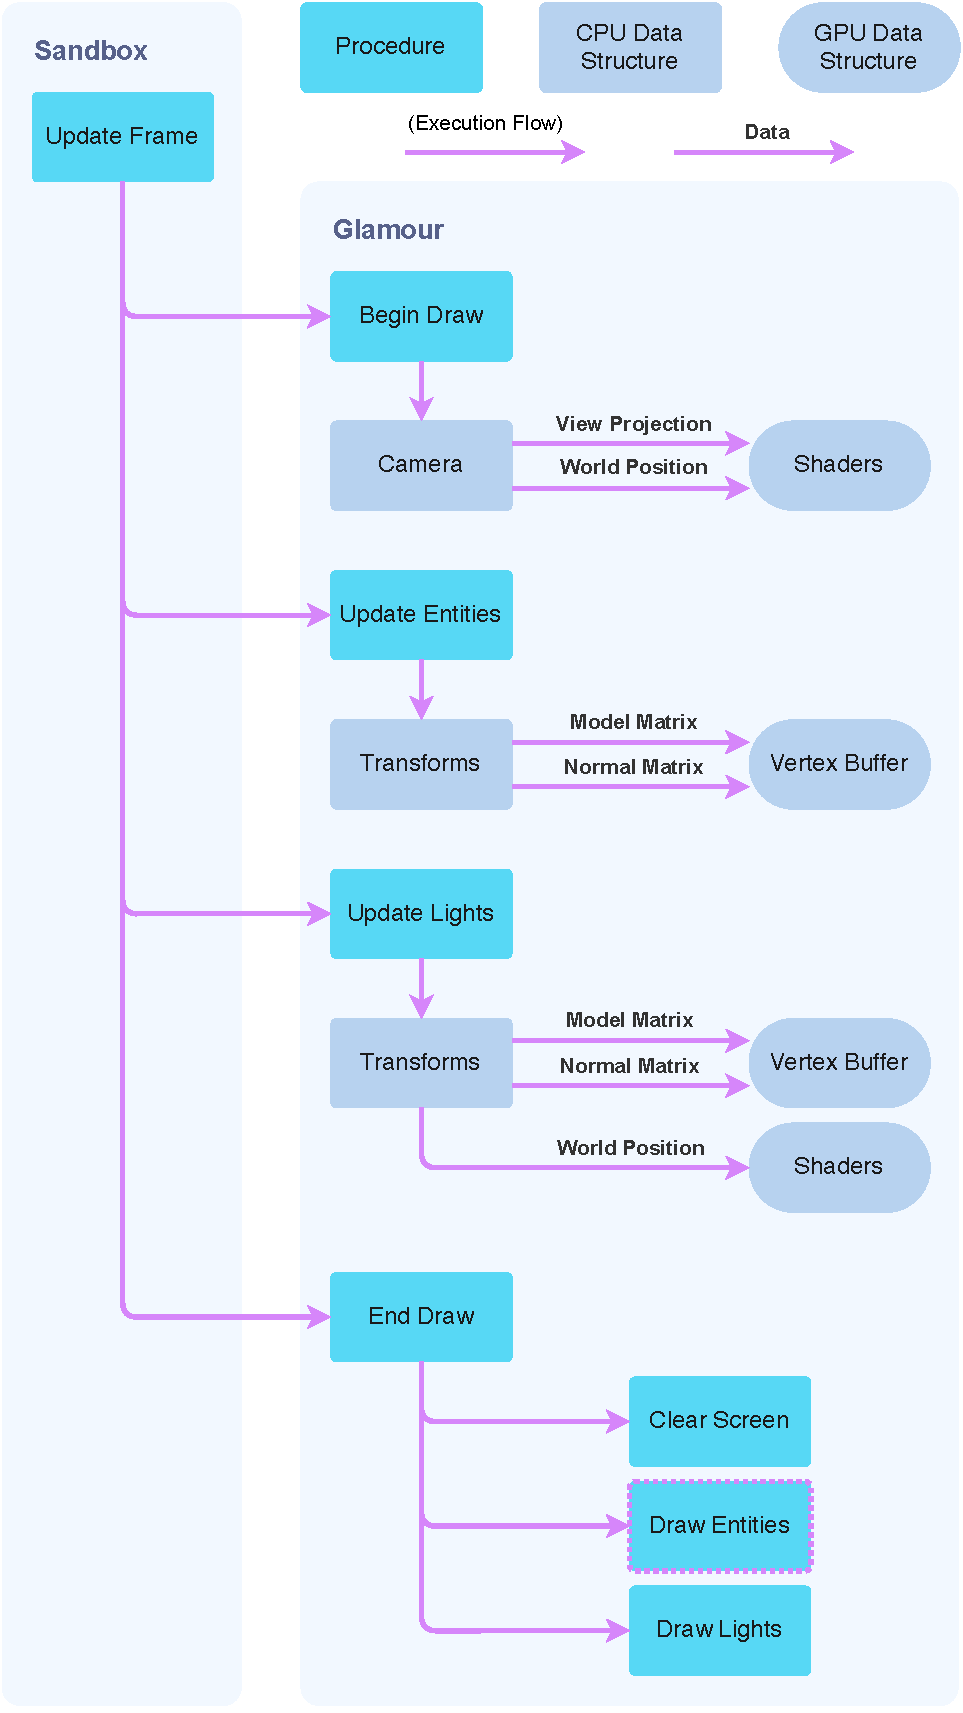
\includegraphics[width=1\columnwidth]{../rendering-pipeline.pdf}
    \caption[Rendering pipeline]{
      \emph{
        The general rendering pipeline.
        \boxy{Draw Entities} is where the difference between forward and deferred is managed.
      }
    }\label{fig:rendering-pipeline}
  \end{figure}

  TODO: Diagram of the rendering pipeline.\\
  Diagram of data structures of \boxy{renderer} and \boxy{SandboxLayer}

  \subsubsection{Forward}
  asdf

  \subsubsection{Deferred}
  asdf

  \subsection{OpenGL}
  abstracting OpenGL and error handling, \boxy{gl_call}.

  \subsection{MVP Transforms}

  \subsubsection{Transform}
  asdf

  \subsubsection{Camera}
  asdf

  \subsection{Shaders}

  \subsubsection{Shader Builder}
  asdf

  \subsubsection{Forward}
  asdf

  \subsubsection{Deferred}
  asdf

  \subsection{Vertex Arrays}
  asdf

  \subsection{Meshes}
  asd

  \subsection{Textures}
  asdf

  \section{Assets}

  \subsection{Asset Management}
  Since Cargo only deals with code, a \boxy{build.rs} script was created to facilitate copying the assets source folder to it's destination directory relative to the built executable.

  There also exists an \boxy{asset} module that exports a helper function \boxy{assets_path()} to obtain the assets directory at runtime, to make loading the assets easier.

  \subsection{Including resources}
  Some files are loaded directly into the application binary at compile time.
  This includes the imgui font and the shaders.
  Rust has a couple of helper macros that make this trivial, namely, \boxy{include_bytes!()} and \boxy{include_str!()}.

  This is something that seems incredibly simple, but cannot be done with just C++ without changing the original file to make it a raw string.
  \emph{50 points to \textbf{Rust}lepuff!}

  \section{Data Collection}

  TODO: Details on how data is collected.

  \section{Tests \& Docs}

  \subsection{Tests}
  The Rust Toolchain comes with built in testing and documentation tool, they can even be combined.
  Now, there aren't a lot of tests in source code at the time of writing, as a lot of it is OpenGL code, which is notoriously hard to ensure robustness because of the multitude of versions and implementations.

  However, a few test experiments were completed as part of a bit of documentation, as rust will compile doc-comment example code and run it as integration tests.

  \subsection{Documentation}
  There also isn't a lot of source code documentation available, but Cargo can generate API documentation from the source code into a web page.

  So, when code is pushed to the GitHub repository, it's built, tested, and the documentation is generated and put up on this website \url{https://glamour.davidjh.com/doc/glamour/index.html}.

  \subsection{Benchmarks}
  Cargo has benchmark tests in nightly preview at the moment, but the \boxy{criterion} crate exists to aid in benchmarking functions in the meantime.

  The benchmarks run a some arbitrary code a bunch of times — generally thousands — and takes a sample of those to compare to the previous run, so the developer can track performance trends.

  These benchmarks have been used to improve the performance of the \boxy{Transform} matrix calculation (which runs thousands of times a frame), and confirm where multi-threading improves performance (mainly by parallelising all those matrix transformations).

  \section{Design Changes}

  TODO: What changed from design to implementation.

  \section{Future Work}

  TODO: Details on issues and improvements that should be addressed, and speculate about other uses for the software.

  \begin{itemize}
    \item Graphics API abstraction, could port to Vulkan/Metal/DirectX/OpenGL-ES
    \item OS Platform abstraction (maybe. glutin/winit handles a lot of that)
    \item Separate window/rendering thread
    \item Vertex Arrays have a lot of nonsense hard coded stuff
    \item G-buffer/frame-buffers could do with a refactor
    \item Shaders should be loaded from disk
    \item Add actual docs, tests, and benchmarks
    \item Once this is an acceptable renderer, I might add more game engine features. Maybe try and make a small game
  \end{itemize}

\end{multicols}

% =================================================================

% \usemintedstyle{manni}
% \begin{minted}{c}
% int main() {
%   printf("hello, world");
%   return 0;
% }
% \end{minted}

% \begin{minted}{rust}
% fn main() {
%   let mut app = App::new("Glamour Sandbox", 512, 490);
%   let sandbox_layer = SandboxLayer::new("SandboxLayer");
%   app.push_layer(Box::new(sandbox_layer));
%   app.run();
% }
% \end{minted}

% \begin{figure}\centering
%   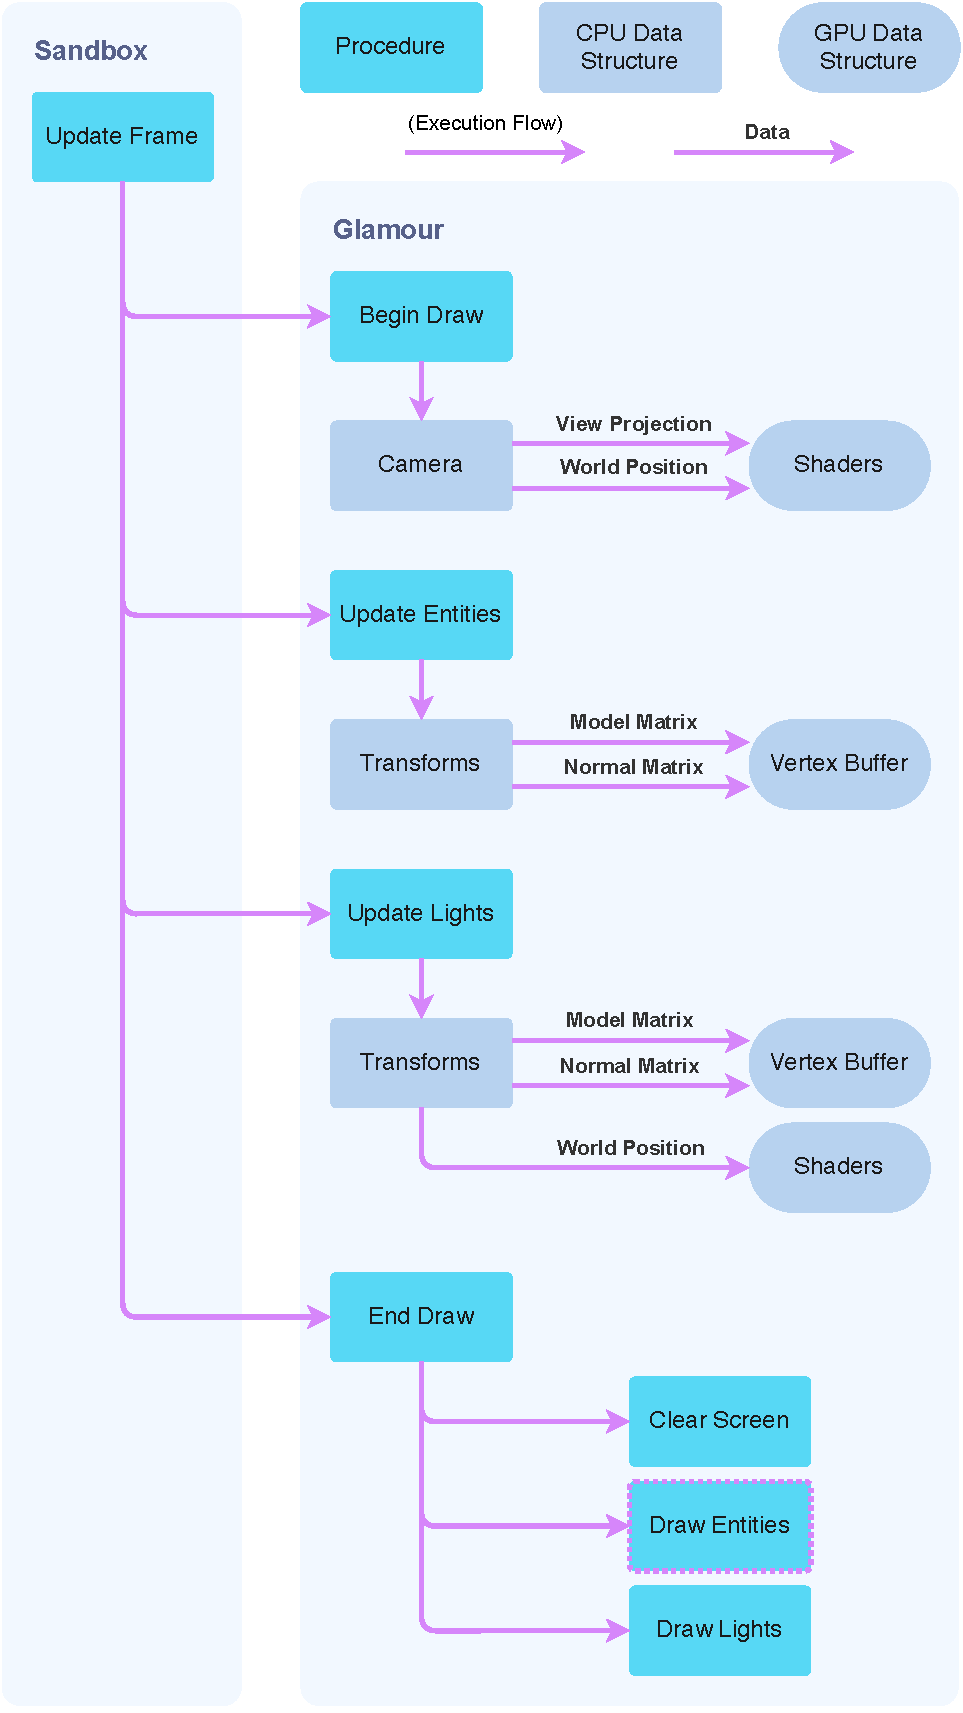
\includegraphics[width=0.7\columnwidth]{../rendering-pipeline.pdf}
%   \caption[Short title]{Long title}\label{fig:ff}
% \end{figure}

\end{document}
